\documentclass[12pt]{beamer}
%\documentclass[20pt,handout]{beamer}
\usetheme{Darmstadt}
\usepackage{graphicx}
\usepackage[german]{babel}
\usepackage[T1]{fontenc}
\usepackage[utf8]{inputenc}
\usepackage{tikz}
\setbeamertemplate{footline}[frame number]

\newcommand{\cc}[1]{\includegraphics[height=4mm]{img/#1.png}}
\usepackage{ifthen}
\newcommand{\license}[2][]{\\#2\ifthenelse{\equal{#1}{}}{}{\\\scriptsize\url{#1}}}
\usepackage{textcomp}

\pgfdeclareimage[height=.6cm]{c3d2logo}{./img/c3d2.pdf} 


\pgfdeclarelayer{foreground}
\pgfsetlayers{main,foreground}
\logo{\pgfputat{\pgfxy(-1,0)}{\pgfbox[center,base]{\pgfuseimage{c3d2logo}}}}


\title{NSA, Prism und co - Wie schützt man sich vor Überwachung?}
\author{\small Marius Melzer \& Stephan Thamm\\\large Chaos Computer Club Dresden}
\date{16.10.2013}

\begin{document}
\maketitle

\section{Einleitung}
\subsection{}

\begin{frame}
  \frametitle{Wer sind wir?}
  \begin{figure}
    
\includegraphics[height=0.7\textheight]{img/fingerabdruck.jpg}
  \end{figure}
\end{frame}

\begin{frame}
  \frametitle{Wer sind wir?}
  \begin{figure}
    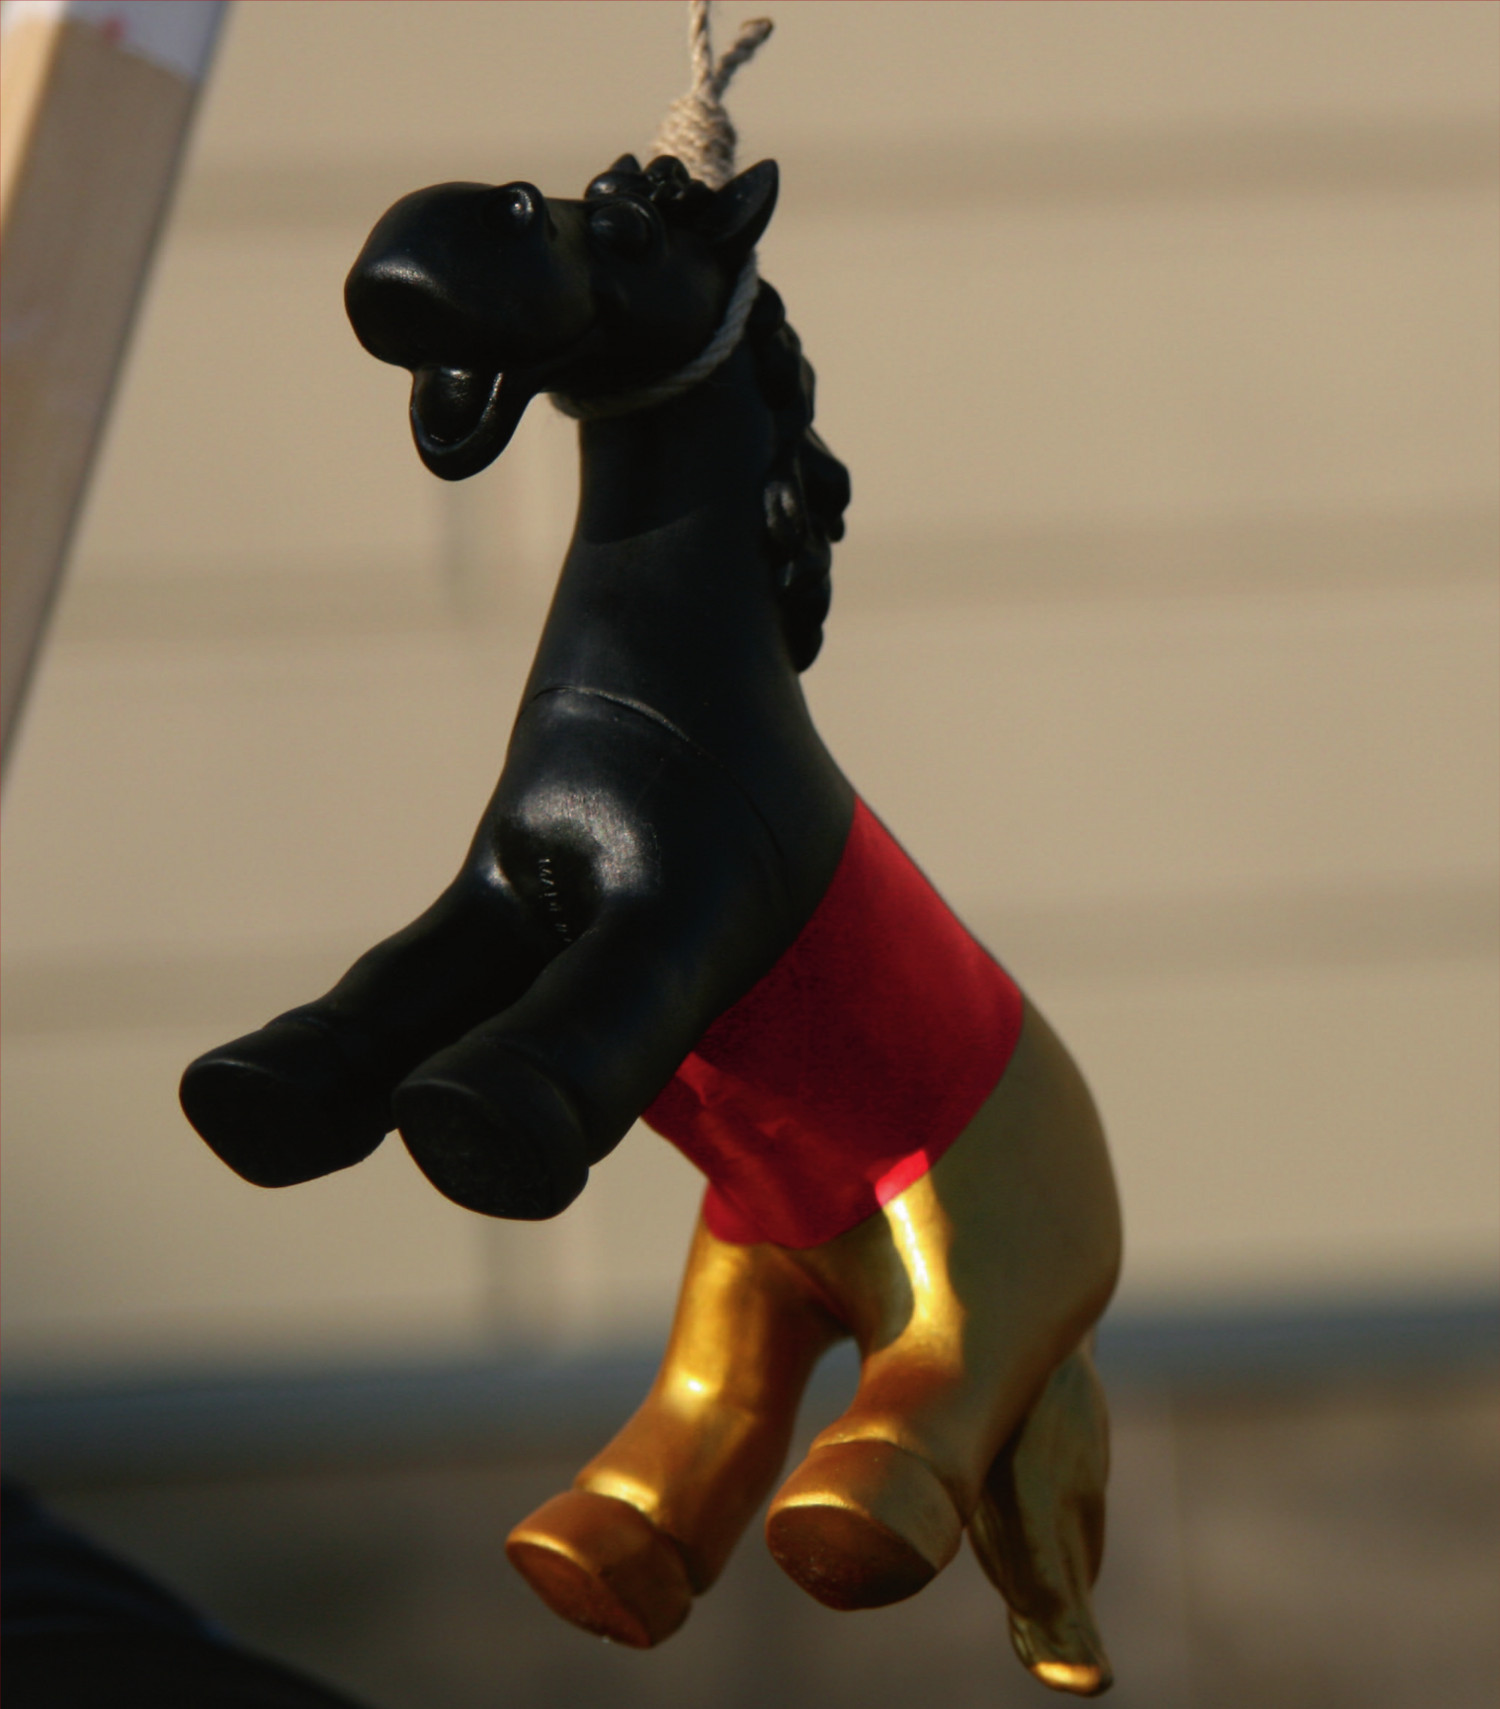
\includegraphics[height=0.7\textheight]{img/trojaner.jpg}
  \end{figure}
\end{frame}

\begin{frame}
    \frametitle{Wer sind wir?}
    \begin{itemize}
      \item<1-> Chaos Computer Club Dresden (\url{http://c3d2.de})
          \note{}
      \item<2-> Datenspuren: Herbst 2014 \url{http://datenspuren.de}
      \item<3-> Podcasts (\url{http://pentamedia.de})
      \item<4-> Chaos macht Schule
    \end{itemize}
\end{frame}

\begin{frame}
    \frametitle{Was ist Sicherheit?}
    \begin{itemize}
      \item<2-> Vertraulichkeit
      \item<3-> Integrität
      \item<4-> Anonymität
    \end{itemize}
\end{frame}

\section{Vertraulichkeit}
\subsection{}

\begin{frame}
    \frametitle{Tempora}
    \begin{itemize}
      \item<2-> britisches GCHQ
      \item<3-> Abhören von Überseekabeln etc.
      \item<4-> Zusammenarbeit mit Firmen
      \item<5-> Keine Unterscheidung zwischen Verdächtigen und Unverdächtigen
    \end{itemize}
\end{frame}

\begin{frame}
    \frametitle{Beispiel Email}
    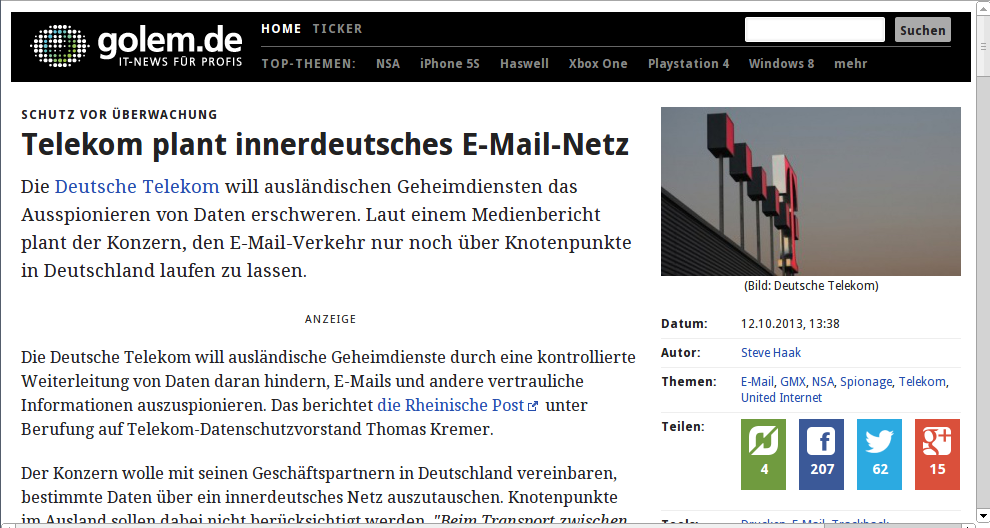
\includegraphics[height=0.7\textheight]{img/telekom_mail.png}<2->
\end{frame}

\begin{frame}
    \frametitle{Beispiel Email}
    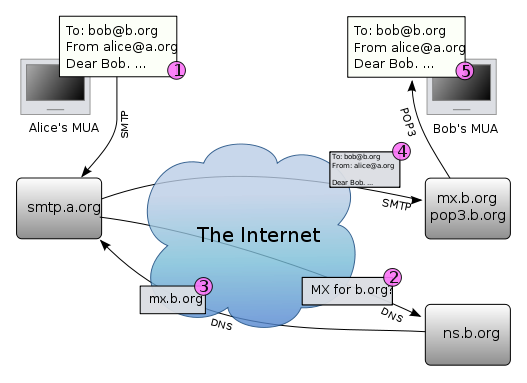
\includegraphics[height=0.7\textheight]{img/527px-Email.png}
\end{frame}

\begin{frame}
    \frametitle{Verschlüsselung}
    \begin{itemize}
      \item<2-> symetrische Verschlüsselung
      \item<3-> asymetrische Verschlüsselung
      \item<4-> Woher kommt Vertrauen?
    \end{itemize}
\end{frame}

\begin{frame}
    \frametitle{SSL / TLS}
    \begin{itemize}
      \item<2-> eingesetzt im Web, Mail, ...
      \item<3-> hierarchische Struktur
      \item<4-> gespeicherte Liste von vertrauenswürdigen Zertifikaten
    \end{itemize}
\end{frame}

\begin{frame}
    \frametitle{GPG / PGP}
    \begin{itemize}
      \item<2-> Ende-zu-Ende Verschlüsselung
      \item<3-> Web of Trust
      \item<4-> Aufbaue eines Netzwerkes aus vertrauenswürdigen Personen
    \end{itemize}
\end{frame}

\begin{frame}
    \frametitle{PRISM}
    \begin{itemize}
      \item<2-> amerikanische NSA
      \item<3-> Zugriff auf Daten bei den Anbietern
      \item<4-> Zusammenarbeit mit Firmen
        \begin{itemize}
          \item<5-> Facebook
          \item<6-> Google
          \item<7-> Microsoft Hotmail
          \item<8-> Skype
          \item<9-> \ldots
        \end{itemize}
    \end{itemize}
\end{frame}

\begin{frame}
    \frametitle{Lavabit}
    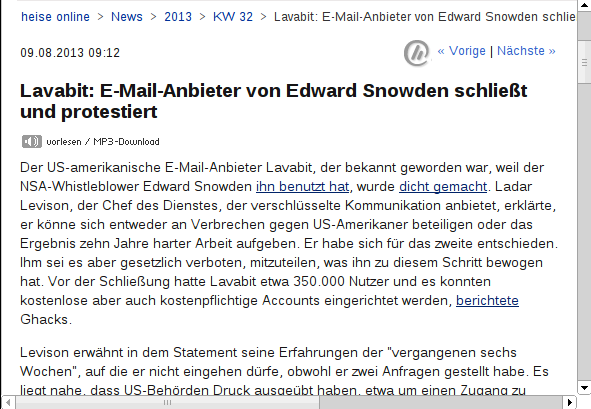
\includegraphics[height=0.6\textheight]{img/heise_lavabit.png}
\end{frame}

\begin{frame}
    \frametitle{Dezentrale Infrastruktur}
    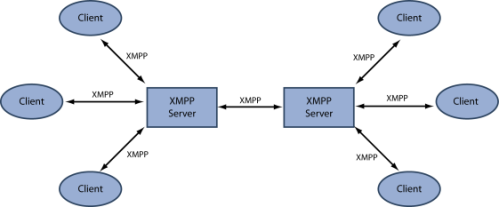
\includegraphics[height=0.5\textheight]{img/xmpp1.png}<2->
\end{frame}

\begin{frame}
    \frametitle{Dezentrale Infrastruktur}
    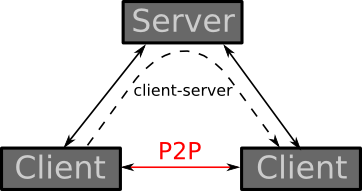
\includegraphics[height=0.5\textheight]{img/client-server-graph.png}
\end{frame}

\begin{frame}
    \frametitle{ZDF Zoom: World Wide War}
\end{frame}

\section{Integrität}
\subsection{}

\begin{frame}
    \frametitle{Infrastruktur}
    Wahrung der Integrität des Netzes möglich durch:
    \begin{itemize}
      \item<1-> Netzneutralität
      \item<2-> Dezentrale, internationale und transparente Aufsicht über Infrastruktur
      \item<3-> Abkommen zu Cyberwar und integrität fremder Netze
    \end{itemize}
\end{frame}

\begin{frame}
    \frametitle{Zensur}
    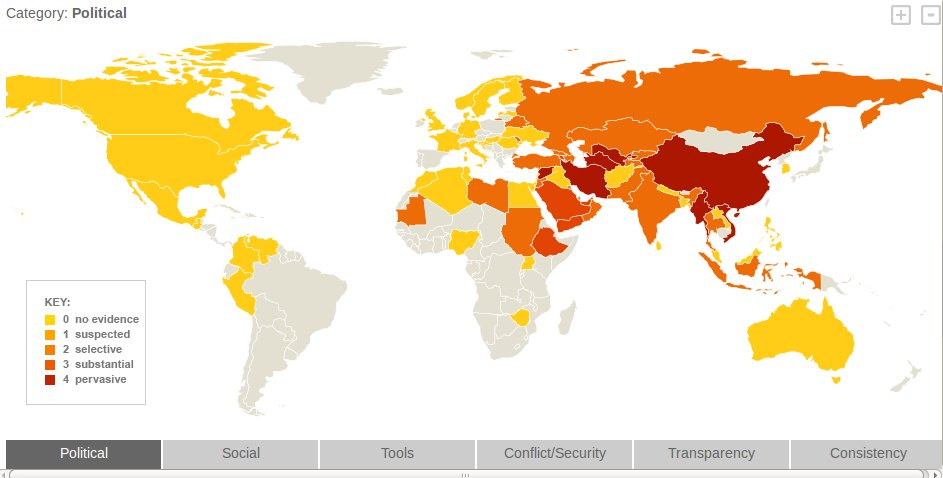
\includegraphics[height=0.7\textheight]{img/zensur-guardian.jpg}
\end{frame}

\begin{frame}
    \frametitle{Arten von Zensur}
    \begin{itemize}
      \item<1-> DNS-basiert
      \item<2-> IP-basiert
      \item<3-> Inhaltsbasiert
    \end{itemize}
\end{frame}

\begin{frame}
    \frametitle{TOR}
    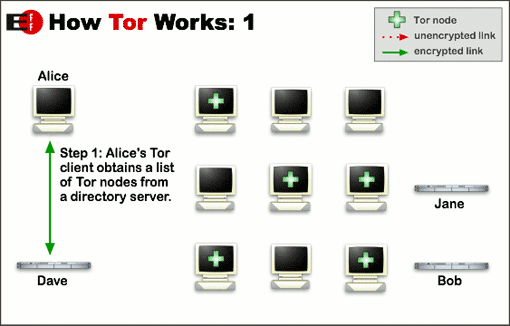
\includegraphics[height=0.7\textheight]{img/tor1.png}
\end{frame}

\begin{frame}
    \frametitle{TOR}
    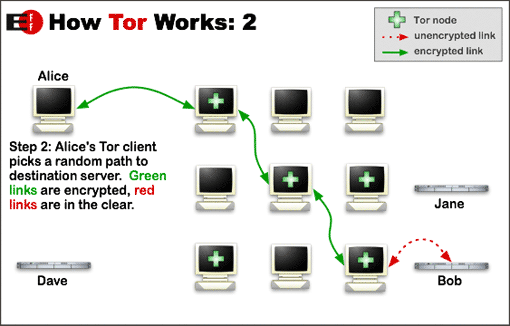
\includegraphics[height=0.7\textheight]{img/tor2.png}
\end{frame}

\begin{frame}
    \frametitle{TOR}
    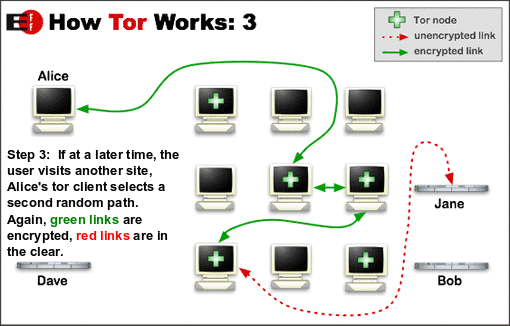
\includegraphics[height=0.7\textheight]{img/tor3.png}
\end{frame}

\begin{frame}
    \frametitle{TOR}
    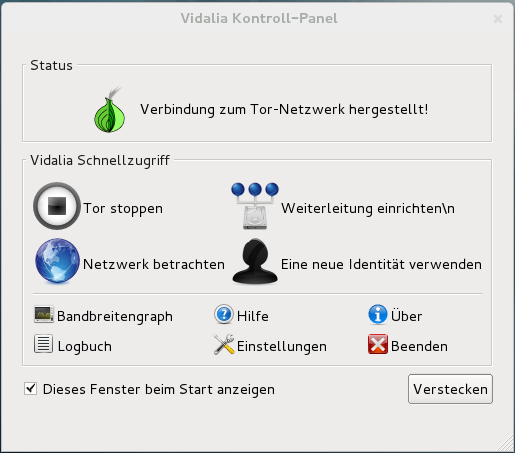
\includegraphics[height=0.7\textheight]{img/vidalia.png}
\end{frame}

\begin{frame}
    \frametitle{TOR}
    \begin{center} \Large Bridges \end{center}
\end{frame}

\begin{frame}
    \frametitle{TOR}
    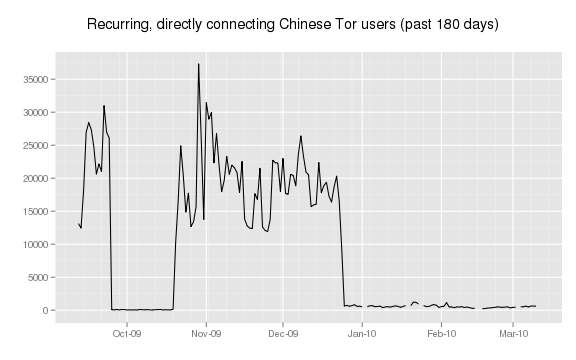
\includegraphics[height=0.7\textheight]{img/bridge1.png}
\end{frame}

\begin{frame}
    \frametitle{TOR}
    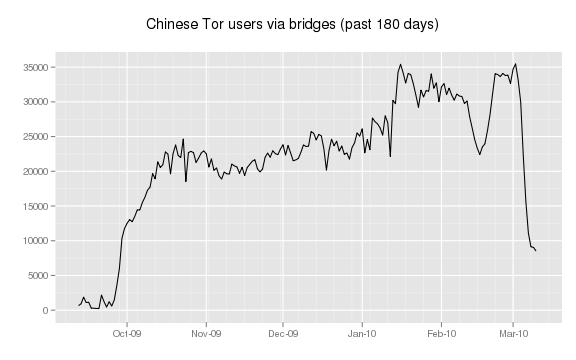
\includegraphics[height=0.7\textheight]{img/bridge2.png}
\end{frame}

\section{Anonymität}
\subsection{}

\begin{frame}
    \frametitle{Metadaten}
    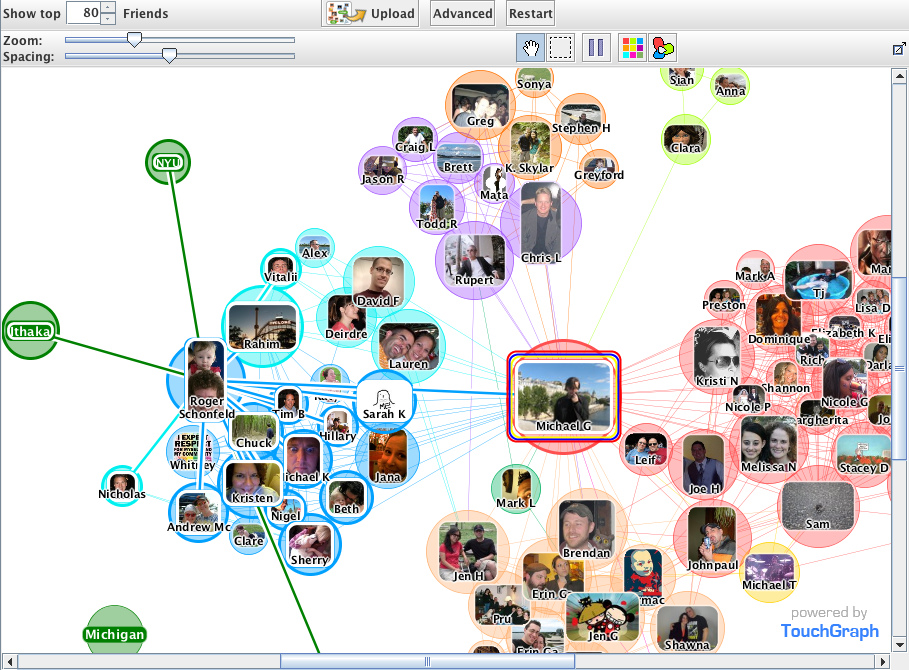
\includegraphics[height=0.7\textheight]{img/socialgraph.jpg}
    \cc{by-sa}
\end{frame}

\begin{frame}
    \frametitle{Metadaten}
    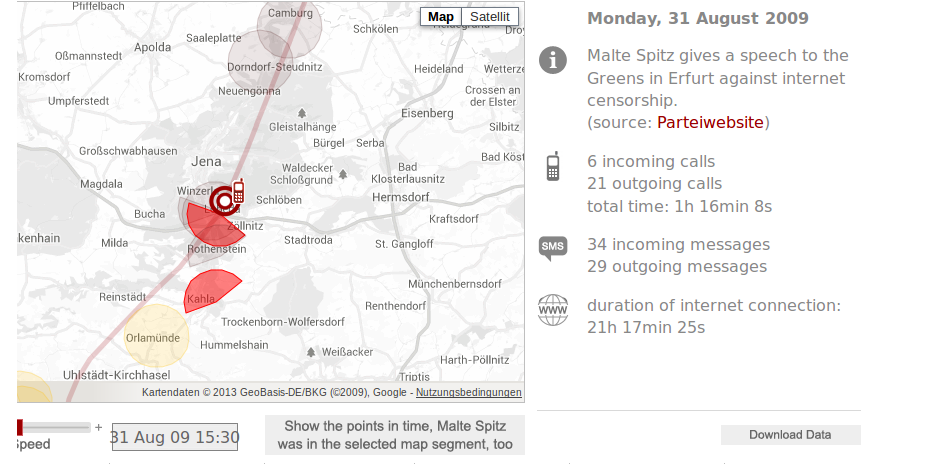
\includegraphics[height=0.7\textheight]{img/maltespitz.png}
\end{frame}

\begin{frame}
    \frametitle{Collusion}
    \begin{center} \Large Collusion \end{center}
\end{frame}

\begin{frame}
    \frametitle{Gegenmaßnahmen}
    \begin{center} \Large Pseudonymität \end{center}
\end{frame}

\begin{frame}
    \frametitle{Gegenmaßnahmen}
    \begin{center} \Large Pseudonymität \end{center}
\end{frame}

\end{document}
